%! Author = user
%! Date = 3/9/2024

% Preamble
\documentclass{article}
\usepackage[utf8]{inputenc}
\usepackage{amsmath, amssymb, amsthm}
\usepackage{tikz}
\usepackage{pgfplots}
\usepackage{listings}
\usepackage[labelformat=empty]{caption}
\usepackage[fontsize=13.5pt]{fontsize}
\usepackage[a4paper,
            bindingoffset=.2in,
            left=.7in,
            right=.7in,
            top=1in,
            bottom=1in,
            footskip=.25in]{geometry}

\definecolor{dkgreen}{rgb}{0,0.6,0}
\definecolor{gray}{rgb}{0.5,0.5,0.5}
\definecolor{mauve}{rgb}{0.58,0,0.82}

\lstset{frame=tb,
  language=Java,
  aboveskip=3mm,
  belowskip=3mm,
  showstringspaces=false,
  columns=flexible,
  basicstyle={\small\ttfamily},
  numbers=none,
  numberstyle=\tiny\color{gray},
  keywordstyle=\color{blue},
  commentstyle=\color{dkgreen},
  stringstyle=\color{mauve},
  breaklines=true,
  breakatwhitespace=true,
  tabsize=3
}

\title{LaTex for Students}
\author{Jun Ho Lee}
\date{March 2024}

% Document
\begin{document}

\newpage
\section{Week4}

Deep Neural Network.

\subsection{Deep L-layer Neural Network}


\begin{figure}[htp]
    \centering
    \begin{minipage}{0.5\textwidth}
        \centering
        \begin{tikzpicture}
            % Input Layer
            \foreach \name/\i in {x1/1,x2/2,x3/3} {
                \node (Input-\i) at (0,-\i) {\name};
                \ifnum \i=1
                    \node[above of=Input-\i] {};
                \fi
            }
            % Hidden Layer
            \foreach \i in {1} {
                \node[circle, minimum size = 7mm, draw=teal!50, line width=.4mm]
                (Hidden1-\i) at (3,-2) {};
                \ifnum \i=1
                \node[above of=Hidden1-\i] {$^{[1]}$};
                \fi
            }
            % Output Layer
            \foreach \name/\i in {$\hat{y}$/1} {
                \node (Output-\i) at (6,-2) {\name};
                \ifnum \i=1
                \node[above of=Output-\i] {};
                \fi
            }
            % Arrows
            \foreach \i in {1,2,3} {
                \foreach \j in {1} {
                \draw[->] (Input-\i) -- (Hidden1-\j);
                }
            }
            \foreach \i in {1} {
                \foreach \j in {1} { \draw[->] (Hidden1-\i) -- (Output-\j);
                }
            }
        \end{tikzpicture}
        \caption{logistic regression}
    \end{minipage}%
    \begin{minipage}{0.5\textwidth}
        \centering
        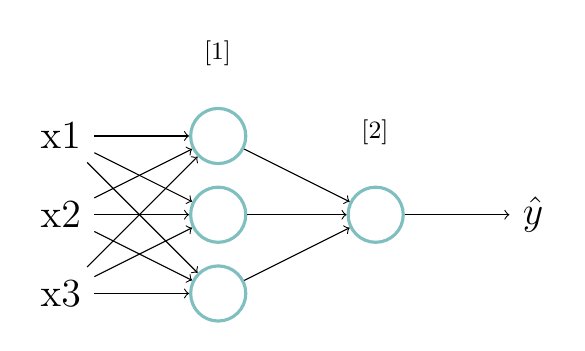
\begin{tikzpicture}
            % Input Layer
            \foreach \name/\i in {x1/1,x2/2,x3/3} {
                \node (Input-\i) at (0,-\i) {\name};
                \ifnum \i=1
                    \node[above of=Input-\i] {};
                \fi
            }
            % Hidden Layer
            \foreach \i in {1,2,3} {
                \node[circle, minimum size = 7mm, draw=teal!50, line width=.4mm]
                (Hidden1-\i) at (2,-\i) {};
                \ifnum \i=1
                \node[above of=Hidden1-\i] {$^{[1]}$};
                \fi
            }
            \foreach \i in {1} {
                \node[circle, minimum size = 7mm, draw=teal!50, line width=.4mm]
                (Hidden2-\i) at (4,-2) {};
                \ifnum \i=1
                \node[above of=Hidden2-\i] {$^{[2]}$};
                \fi
            }
            % Output Layer
            \foreach \name/\i in {$\hat{y}$/1} {
                \node (Output-\i) at (6,-2) {\name};
                \ifnum \i=1
                \node[above of=Output-\i] {};
                \fi
            }
            % Arrows
            \foreach \i in {1,2,3} {
                \foreach \j in {1,2,3} {
                \draw[->] (Input-\i) -- (Hidden1-\j);
                }
            }
            \foreach \i in {1,2,3} {
                \foreach \j in {1} {
                \draw[->] (Hidden1-\i) -- (Hidden2-\j);
                }
            }
            \foreach \i in {1} {
                \foreach \j in {1} { \draw[->] (Hidden2-\i) -- (Output-\j);
                }
            }
        \end{tikzpicture}
        \caption{2-Layer}
    \end{minipage}
    \begin{minipage}{0.5\textwidth}
        \centering
        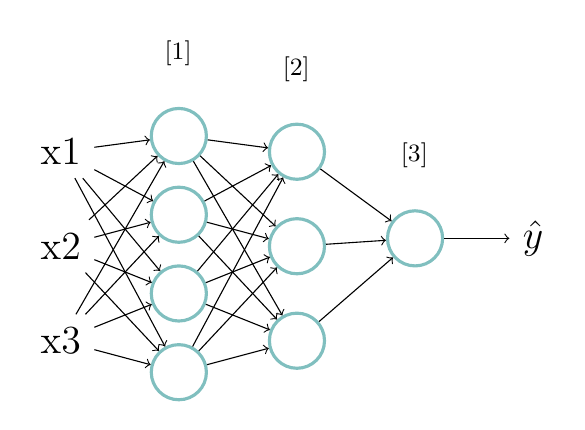
\begin{tikzpicture}
            % Input Layer
            \foreach \name/\i in {x1/1,x2/2,x3/3} {
                \node (Input-\i) at (0,-\i*1.2) {\name};
                \ifnum \i=1
                    \node[above of=Input-\i] {};
                \fi
            }
            % Hidden Layer
            \foreach \i in {1,2,3,4} {
                \node[circle, minimum size = 7mm, draw=teal!50, line width=.4mm]
                (Hidden1-\i) at (1.5,-\i) {};
                \ifnum \i=1
                \node[above of=Hidden1-\i] {$^{[1]}$};
                \fi
            }
            \foreach \i in {1,2,3} {
                \node[circle, minimum size = 7mm, draw=teal!50, line width=.4mm]
                (Hidden2-\i) at (3,-\i*1.2) {};
                \ifnum \i=1
                \node[above of=Hidden2-\i] {$^{[2]}$};
                \fi
            }
            \foreach \i in {1} {
                \node[circle, minimum size = 7mm, draw=teal!50, line width=.4mm]
                (Hidden3-\i) at (4.5,-2.3) {};
                \ifnum \i=1
                \node[above of=Hidden3-\i] {$^{[3]}$};
                \fi
            }
            % Output Layer
            \foreach \name/\i in {$\hat{y}$/1} {
                \node (Output-\i) at (6,-2.3) {\name};
                \ifnum \i=1
                \node[above of=Output-\i] {};
                \fi
            }
            % Arrows
            \foreach \i in {1,2,3} {
                \foreach \j in {1,2,3,4} {
                \draw[->] (Input-\i) -- (Hidden1-\j);
                }
            }
            \foreach \i in {1,2,3,4} {
                \foreach \j in {1,2,3} {
                \draw[->] (Hidden1-\i) -- (Hidden2-\j);
                }
            }
            \foreach \i in {1,2,3} {
                \foreach \j in {1} {
                \draw[->] (Hidden2-\i) -- (Hidden3-\j);
                }
            }
            \foreach \i in {1} {
                \foreach \j in {1} { \draw[->] (Hidden3-\i) -- (Output-\j);
                }
            }
        \end{tikzpicture}
        \caption{3-Layer}
    \end{minipage}%
    \begin{minipage}{0.5\textwidth}
        \centering
        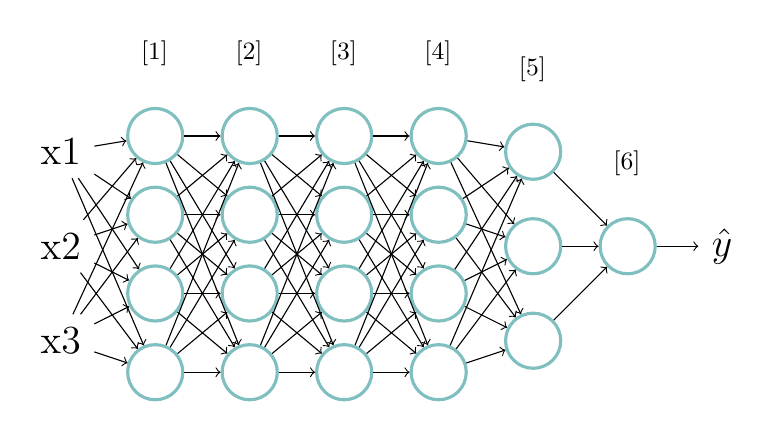
\begin{tikzpicture}
            % Input Layer
            \foreach \name/\i in {x1/1,x2/2,x3/3} {
                \node (Input-\i) at (0,-\i*1.2) {\name};
                \ifnum \i=1
                    \node[above of=Input-\i] {};
                \fi
            }
            % Hidden Layer
            \foreach \i in {1,2,3,4} {
                \node[circle, minimum size = 7mm, draw=teal!50, line width=.4mm]
                (Hidden1-\i) at (1.2,-\i) {};
                \ifnum \i=1
                \node[above of=Hidden1-\i] {$^{[1]}$};
                \fi
            }
            \foreach \i in {1,2,3,4} {
                \node[circle, minimum size = 7mm, draw=teal!50, line width=.4mm]
                (Hidden2-\i) at (2.4,-\i) {};
                \ifnum \i=1
                \node[above of=Hidden2-\i] {$^{[2]}$};
                \fi
            }
            \foreach \i in {1,2,3,4} {
                \node[circle, minimum size = 7mm, draw=teal!50, line width=.4mm]
                (Hidden3-\i) at (3.6,-\i) {};
                \ifnum \i=1
                \node[above of=Hidden3-\i] {$^{[3]}$};
                \fi
            }
            \foreach \i in {1,2,3,4} {
                \node[circle, minimum size = 7mm, draw=teal!50, line width=.4mm]
                (Hidden4-\i) at (4.8,-\i) {};
                \ifnum \i=1
                \node[above of=Hidden4-\i] {$^{[4]}$};
                \fi
            }
            \foreach \i in {1,2,3} {
                \node[circle, minimum size = 7mm, draw=teal!50, line width=.4mm]
                (Hidden5-\i) at (6,-\i*1.2) {};
                \ifnum \i=1
                \node[above of=Hidden5-\i] {$^{[5]}$};
                \fi
            }
            \foreach \i in {1} {
                \node[circle, minimum size = 7mm, draw=teal!50, line width=.4mm]
                (Hidden6-\i) at (7.2,-2.4) {};
                \ifnum \i=1
                \node[above of=Hidden6-\i] {$^{[6]}$};
                \fi
            }
            % Output Layer
            \foreach \name/\i in {$\hat{y}$/1} {
                \node (Output-\i) at (8.4,-2.4) {\name};
                \ifnum \i=1
                \node[above of=Output-\i] {};
                \fi
            }
            % Arrows
            \foreach \i in {1,2,3} {
                \foreach \j in {1,2,3,4} {
                \draw[->] (Input-\i) -- (Hidden1-\j);
                }
            }
            \foreach \i in {1,2,3,4} {
                \foreach \j in {1,2,3,4} {
                \draw[->] (Hidden1-\i) -- (Hidden2-\j);
                }
            }
            \foreach \i in {1,2,3,4} {
                \foreach \j in {1,2,3,4} {
                \draw[->] (Hidden2-\i) -- (Hidden3-\j);
                }
            }
            \foreach \i in {1,2,3,4} {
                \foreach \j in {1,2,3,4} {
                \draw[->] (Hidden3-\i) -- (Hidden4-\j);
                }
            }
            \foreach \i in {1,2,3,4} {
                \foreach \j in {1,2,3} {
                \draw[->] (Hidden4-\i) -- (Hidden5-\j);
                }
            }
            \foreach \i in {1,2,3} {
                \foreach \j in {1} { \draw[->] (Hidden5-\i) -- (Hidden6-\j);
                }
            }
            \foreach \i in {1} {
                \foreach \j in {1} { \draw[->] (Hidden6-\i) -- (Output-\j);
                }
            }
        \end{tikzpicture}
        \caption{6-Layer}
    \end{minipage}
    \caption{Neural network with different hidden layers}
\end{figure}


\newpage

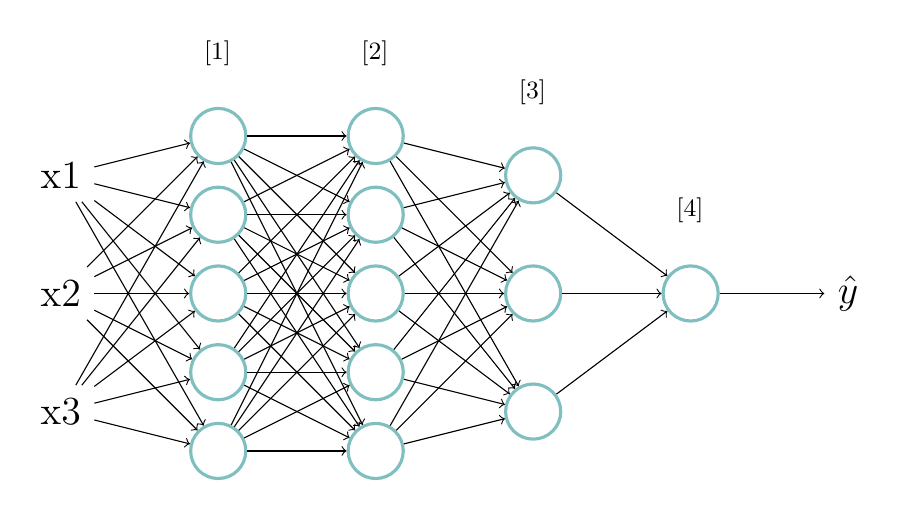
\begin{tikzpicture}
% Input Layer
\foreach \name/\i in {x1/1,x2/2,x3/3} {
    \node (Input-\i) at (0,-\i*1.5) {\name};
    \ifnum \i=1
        \node[above of=Input-\i] {};
    \fi
}
% Hidden Layer
\foreach \i in {1,2,3,4,5} {
    \node[circle, minimum size = 7mm, draw=teal!50, line width=.4mm]
    (Hidden1-\i) at (2,-\i) {};
    \ifnum \i=1
    \node[above of=Hidden1-\i] {$^{[1]}$};
    \fi
}
\foreach \i in {1,2,3,4,5} {
    \node[circle, minimum size = 7mm, draw=teal!50, line width=.4mm]
    (Hidden2-\i) at (4,-\i) {};
    \ifnum \i=1
    \node[above of=Hidden2-\i] {$^{[2]}$};
    \fi
}
\foreach \i in {1,2,3} {
    \node[circle, minimum size = 7mm, draw=teal!50, line width=.4mm]
    (Hidden3-\i) at (6,-\i*1.5) {};
    \ifnum \i=1
    \node[above of=Hidden3-\i] {$^{[3]}$};
    \fi
}
\foreach \i in {1} {
    \node[circle, minimum size = 7mm, draw=teal!50, line width=.4mm]
    (Hidden4-\i) at (8,-3) {};
    \ifnum \i=1
    \node[above of=Hidden4-\i] {$^{[4]}$};
    \fi
}
% Output Layer
\foreach \name/\i in {$\hat{y}$/1} {
    \node (Output-\i) at (10,-3) {\name};
    \ifnum \i=1
    \node[above of=Output-\i] {};
    \fi
}
% Arrows
\foreach \i in {1,2,3} {
    \foreach \j in {1,2,3,4,5} {
    \draw[->] (Input-\i) -- (Hidden1-\j);
    }
}
\foreach \i in {1,2,3,4,5} {
    \foreach \j in {1,2,3,4,5} {
    \draw[->] (Hidden1-\i) -- (Hidden2-\j);
    }
}
\foreach \i in {1,2,3,4,5} {
    \foreach \j in {1,2,3} {
    \draw[->] (Hidden2-\i) -- (Hidden3-\j);
    }
}
\foreach \i in {1,2,3} {
    \foreach \j in {1} {
    \draw[->] (Hidden3-\i) -- (Hidden4-\j);
    }
}
\foreach \i in {1} {
    \foreach \j in {1} { \draw[->] (Hidden4-\i) -- (Output-\j);
    }
}
\end{tikzpicture}

$L=4 = $ Total number of layers.\\

$X = a^{[0]}$\\

$\hat{y} = a^{[L]}$\\

$n^{[l]} = $ number of units in layer $l$\\

$a^{[l]} = g^{[l]}(z^{[l]})= $ activation in layer $l$\\

$W^{[l]}= $ weights for $Z^{[l]}$\\

$b^{[l]}= $ bias for $Z^{[l]}$\\

$_{n^{[0]} = n_x = 3, \hspace{2mm} n^{[1]} = 5, \hspace{2mm} n^{[2]} = 5, \hspace{2mm} n^{[3]} = 3, \hspace{2mm} n^{[4]} = n^{[L]} = 1}$\\

\newpage
\subsection{Forward Propagation in a deep network}

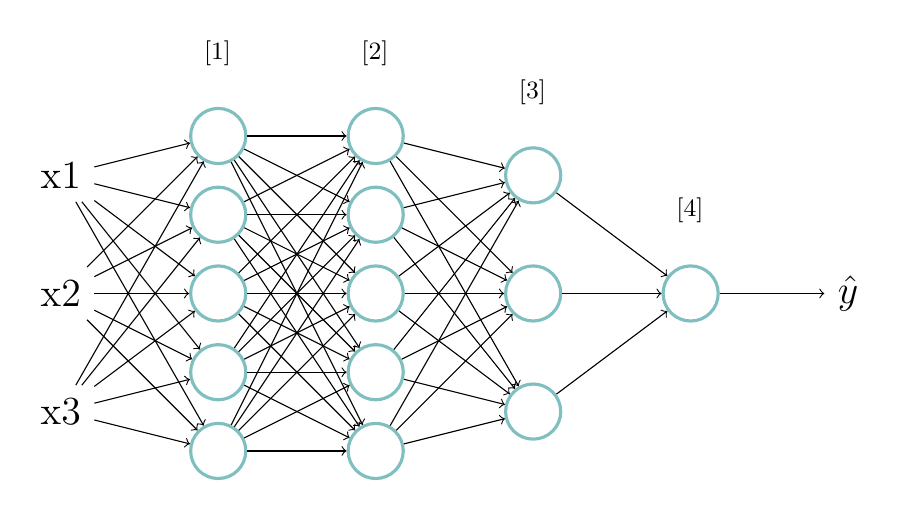
\begin{tikzpicture}
% Input Layer
\foreach \name/\i in {x1/1,x2/2,x3/3} {
    \node (Input-\i) at (0,-\i*1.5) {\name};
    \ifnum \i=1
        \node[above of=Input-\i] {};
    \fi
}
% Hidden Layer
\foreach \i in {1,2,3,4,5} {
    \node[circle, minimum size = 7mm, draw=teal!50, line width=.4mm]
    (Hidden1-\i) at (2,-\i) {};
    \ifnum \i=1
    \node[above of=Hidden1-\i] {$^{[1]}$};
    \fi
}
\foreach \i in {1,2,3,4,5} {
    \node[circle, minimum size = 7mm, draw=teal!50, line width=.4mm]
    (Hidden2-\i) at (4,-\i) {};
    \ifnum \i=1
    \node[above of=Hidden2-\i] {$^{[2]}$};
    \fi
}
\foreach \i in {1,2,3} {
    \node[circle, minimum size = 7mm, draw=teal!50, line width=.4mm]
    (Hidden3-\i) at (6,-\i*1.5) {};
    \ifnum \i=1
    \node[above of=Hidden3-\i] {$^{[3]}$};
    \fi
}
\foreach \i in {1} {
    \node[circle, minimum size = 7mm, draw=teal!50, line width=.4mm]
    (Hidden4-\i) at (8,-3) {};
    \ifnum \i=1
    \node[above of=Hidden4-\i] {$^{[4]}$};
    \fi
}
% Output Layer
\foreach \name/\i in {$\hat{y}$/1} {
    \node (Output-\i) at (10,-3) {\name};
    \ifnum \i=1
    \node[above of=Output-\i] {};
    \fi
}
% Arrows
\foreach \i in {1,2,3} {
    \foreach \j in {1,2,3,4,5} {
    \draw[->] (Input-\i) -- (Hidden1-\j);
    }
}
\foreach \i in {1,2,3,4,5} {
    \foreach \j in {1,2,3,4,5} {
    \draw[->] (Hidden1-\i) -- (Hidden2-\j);
    }
}
\foreach \i in {1,2,3,4,5} {
    \foreach \j in {1,2,3} {
    \draw[->] (Hidden2-\i) -- (Hidden3-\j);
    }
}
\foreach \i in {1,2,3} {
    \foreach \j in {1} {
    \draw[->] (Hidden3-\i) -- (Hidden4-\j);
    }
}
\foreach \i in {1} {
    \foreach \j in {1} { \draw[->] (Hidden4-\i) -- (Output-\j);
    }
}
\end{tikzpicture}\\

$Z^{[1]} = W^{[1]} A^{[0]} + b^{[1]} _{\hspace{5mm} where \hspace{1mm} A^{[0]} = X}$\\

$A^{[1]} = g^{[{1}]} (Z^{[1]})$\\

$Z^{[2]} = W^{[2]} A^{[1]} + b^{[2]}$\\

$A^{[2]} = g^{[{2}]} (Z^{[2]})$\\

\dots \\

$Z^{[4]} = W^{[4]} A^{[3]} + b^{[4]}$\\

$A^{[4]} = g^{[{4}]} (Z^{[4]}) = \hat{Y}$\\

\noindent\rule{8cm}{0.4pt}

Using for loops on $[l]$ layer for $l=1,2,\dots, L$:\\

$Z^{[l]} = W^{[l]} A^{[l-1]} + b^{[l]}$\\

$A^{[l]} = g^{[{l}]} (Z^{[l]})$\\

\newpage
\subsection{Getting Matrix Dimensions Right}

For a single training example:\\

$Z^{[l]} = W^{[l]} A^{[l-1]} + b^{[l]}$\\
$\indent$ $_{(n^{[l]},1) = (n^{[l]},n^{[l-1]}) \times (n^{[l-1]},1) + (n^{[l]},1))}$\\

$A^{[l]} = g^{[{l}]} (Z^{[l]})$\\

\noindent\rule{8cm}{0.4pt}

For $m$ training examples:\\

$Z^{[l]} = W^{[l]} A^{[l-1]} + b^{[l]}$\\

$A^{[l]} = g^{[{l}]} (Z^{[l]})$\\

$dZ^{[l]}, \hspace{2mm} dA^{[l]}$\\
$\indent$ $_{(n^{[l]},m) = (n^{[l]},n^{[l-1]}) \times (n^{[l-1]},m) +(n^{[l]},1), \hspace{3mm} \text{where} \hspace{1mm} b^{[l]} \hspace{1mm} \text{is broadcasted to} \hspace{1mm} (n^{[l]},m)}$\\


\newpage
\subsubsection{Why Deep Representations?}

Intuition about deep representation:
Each layer could be edge dectector, facial detector, etc going from lower to deeper layers.
Simple to complex hierarchical representation(compositional) could be applied to other types of data.(image, audio, ...).


Circuit theory and deep learning: Informally: There are functions you can compute with a "small" L-layer deep neural network that shallower networks require exponentially more hidden units to compute.

\newpage
\subsection{Building Blocks of a Deep Neural Network}

$\indent$ Forward:\\

$a^{{[l-1]}} \rightarrow w^{[l]}, b^{[l]} \rightarrow a^{{[l]}}, \hspace{1mm} _{\text{cache}} \hspace{1mm} z^{[l]}$\\


Backward:\\

$da^{{[l-1]}}, dw^{[l]}, db^{[l]}, dz^{[l]} \leftarrow w^{[l]}, b^{[l]}, dz^{[l]} \leftarrow da^{{[l]}}$\\


Update parameters:\\

$w^{[l]} = w^{[l]} - \alpha dw^{[l]}$\\

$b^{[l]} = b^{[l]} - \alpha db^{[l]}$\\


\newpage
\subsection{Forward and Backward Propagation}


$\indent$ Forward propagation for layer $l$: $a^{[l-1]}\rightarrow a^{[l]}, z^{[l]}, w^{[l]}, b^{[l]}$\\

$Z^{[l]} = W^{[l]} A^{[l-1]} + b^{[l]}$\\

$A^{[l]} = g^{[l]} (Z^{[l]})$\\

(for $i=1,\dots,L$ with initial value $A^{[0]} = X$)\\

Backward propagation for layer $l$: $da^{[l]} \rightarrow da^{[l-1]},dW^{[l]}, db^{[l]}$\\

$dZ^{[l]} = dA^{[l]} * {g^{[l]}}^{'}(Z^{[l]})$\\

$dW^{[l]} = \frac{1}{m}dZ^{[l]}{A^{[l-1]}}^T$\\

$db^{[l]} = \frac{1}{m}np.sum(dZ^{[l]}, axis=1, keepdims=True)$\\

$dA^{[l-1]} = {W^{[l]}}^T dZ^{[l]} = \frac{dJ}{dA^{[l-1]}} = \frac{dZ^{[l]}}{dA^{[l-1]}} \frac{dJ}{dZ^{[l]}} = \frac{dZ^{[l]}}{dA^{[l-1]}} dZ^{[l]}$\\

(with initial value $dZ^{[L]} = A^{[L]}-Y$)\\



\newpage
\subsection{Parameter vs. Hyperparameter}

$\indent$ Paramters: $W^{[l]}, b^{[l]}$\\

Hyperparameters: $_{\text{(it affects paramters)}}$\\

$\indent$ learning rate $\alpha$\\

$\indent$ number of iterations \\

$\indent$ number of hidden layers $L$\\

$\indent$ number of hidden units $n^{[l]}$\\

$\indent$ Choice of activation function\\

$\indent$ later: Momentum, minibatch size, regularization paramters, ...\\


\subsubsection*{Applied deep learning is a very empirical process}

$\indent$ Idea, Code, Experiment\\

number of iterations $\rightarrow$ cost $J$ decreases.\\


\newpage
\subsection{What does this have to do with the brain?}


\end{document}

